\section{Ejercicio 2}

\subsection{Introducción}

\paragraph{}
En esta sección se presentara un algoritmo exacto para resolver el problema de encontrar la Clique Máxima en un grafo.


\paragraph{}
Aun no se conocen algoritmos buenos, es decir, polinomiales con respecto al tamaño de la entrada, para resolver 
este problema, asi que nos consentraremos en realizar mejoras al algoritmo de fuerza bruta que considera todos los casos.


\subsection{Explicación}

\paragraph{}
Un algoritmo de fuerza bruta para resolver el problema de Max-Clique podría simplemente intentar formar el conjunto más 
grande de nodos, donde ese conjunto sea completo, intentando todas las posibilidades eligiendo todos los conjuntos de un cierto tamaño,
luego intentar con un tamaño menor, etc. Probablemente la complejidad de un algoritmo de este estilo sea $n^n$ donde n es la cantidad 
de nodos del grafo.

\paragraph{}
Una mejora que surge casi inmediatamente es utilizar la técnica de BackTracking, cuya función principal es intentar podar el 
arbol implicito de combinaciones posibles. 

\paragraph{}
De todas maneras, implementar solo un BackTracking parece ser poco con respecto a las mejoras que se pueden lograr. A continuación, 
se explicara el algoritmo implementado con un pseudocodigo y se verá cada una de las mejoras por separado.
\vspace{2em}
\incmargin{3em}
\linesnumbered
\restylealgo{boxed}
\footnotesize 
\textbf{Algoritmo Exacto}(G: grafo) \\
\begin{algorithm}[H]
	\BlankLine
		CliqueMayor = vacia\\
		componentesConexas = DetectarComponentesConexas(G)
		\BlankLine

		\textbf{Para cada} componente \textbf{en} componentesConexas \{ 
		\BlankLine

		\tab\tab heap = crearHeap(G,componentes) \\

		\BlankLine
		\tab\tab \textbf{Mientras} noVacio(heap) $\wedge$ top(heap) $\geq$ tam(CliqueMayorActual)\{\\
		\BlankLine
		\tab\tab\tab v = top(heap)
		\BlankLine
		\tab\tab\tab \textbf{Para} tamCliqueABuscar \textbf{desde} grado(v)+1 \textbf{hasta} tam(CliqueMayorActual)+1\{\\
		\tab\tab\tab\tab vecinosFiltrados = 	filtrarVecinosMenores(v, tamCliqueABuscar-1)\\						
		\tab\tab\tab\tab \textbf{Si} tam(vecinosFiltrados) +1 $\geq$ tamCliqueABuscar\\ 			
		\tab\tab\tab\tab\tab temp = BuscoCliqueDeTamañoK(tamCliqueABuscar, vecinosFiltrados)
		\BlankLine
		\tab\tab\tab\tab\tab \textbf{Si}  tam(CliqueMayorActual)  $<$ tam(temp)\\ 
		\tab\tab\tab\tab\tab\tab CliqueMayorActual  = temp\\
		\tab\tab\tab\}\\
		\tab\tab\}
\caption{Pseudocódigo del algoritmo exacto}
\end{algorithm}

\normalsize

\paragraph{}
Primero, se detectan las componentes conexas del grafo, ya que buscar la max clique en todo el grafo es equivalente a quedarse con la máxima de las max cliques de cada componente conexa.

\paragraph{}
Luego, para cada componente, se crea un heap que contiene los nodos de la componente ordenados por mayor grado. Esto no parece tener mucha importancia, pero se aclarará a medida que se avanza con la explicación.

\paragraph{}
A partir de esta estructura, vamos obteniendo en cada iteración, el nodo $v$ de mayor grado disponible en la componente que no hayamos analizado.

\paragraph{}
Una vez que tenemos el nodo $v$, lo que se hace es buscar la mayor clique en la cual está contenido. Para ello utilizamos la función BuscoCliqueDeTamañoK a la cual le indicamos el tamaño de la clique que queremos buscar (buscaremos cliques de tamaños desde el grado de $v$ + 1 hasta el de la clique que ya hemos encontrado sin incluir, ya que el resto de los resultados no nos serían de utilidad) y los vecinos de $v$ que tienen posibilidades de pertenecer a la clique (dado su grado).

\paragraph{}
Por ejemplo, veamos la siguiente figura:

\includegraphics[scale = 0.9]{./p.ps} \\

\paragraph{}
Como se ve en el ejemplo, 


